
Machine learning techniques can be broadly grouped into 4 categories based on the types of problems they solve. \textbf{Clustering} problems try to find groupings in data sets by minimizing distances from members of the same group and maximizing distances between members of differing groups. \textbf{Classification} problems map new instance data onto a discrete set of values representing categories or labels, while \textbf{regression} maps new data onto a continuous set of values. \textbf{Rule extraction}\cite{Denker} is a statistical inference method used to predict responses from given input patterns. It is also common to describe machine learning by one of four types of learning used. \textbf{Supervised} learning is provided labeled training data to build models from, while \textbf{unsupervised} learning is trained on unlabeled data. \textbf{Semi-supervised} learning is used with a mix of labeled and unlabeled data. \textbf{Reinforcement} learning\cite{Sutton_Barto_2018} maximizes values from an internal scoring functions to learn a model about the environment. 

The use of machine learning techniques in cyber security is just starting to be explored. The two surveys\cite{Buczak_Guven_2016, Xin_Kong_Liu_Chen_Li_Zhu_Gao_Hou_Wang_2018} published in 2016 and 2018 review a wide range of ML and RL methods specific to the area of intrusion detection. In \cite{Boutaba_2018} the authors survey the field of networking generally for uses of machine learning. Their findings cover areas in traffic management like routing and congestion control, as well as resource and fault management topics. On the subject of network security, the subject areas reviewed were again narrowly focused on intrusion detection. 

In this work we describe methods for evaluating cyber security that incorporate the underlying structure of the (computer) network under test. Graphs are a natural way to represent network connections and the relationships between system components, but preserving that structure adds complexity to the cost of analysis. Modern machine learning techniques make use of optimizations and transformations to reduce their complexity, and graph learning methods are no exception. Similar to preprocessing an image set to uniform dimensions prior to training, many graph learning methods presuppose an embedding of the graph data as input requirement. Goyal’s graph embedding survey\cite{Goyal_Ferrara_2018} finds 4 broad categories of these methods:
\begin{enumerate}
\item \textbf{Node Classification}: Predict the label of a node based on its embedding. 
\item \textbf{Link Predicton}: Predict edge based on embeddings of nodes it joins.
\item \textbf{Clustering}: Community detections and node groupings.
\item \textbf{Visualization}: Interpreting more than a few dozen nodes becomes difficult. 
\end{enumerate}

Graph embedding can mean either embedding the entire graph in vector space, or embedding each node in vector space. The goal in either case is to encode the graph data onto a lower dimensional space while retaining the relevant structural relationships. Common practice is to learn graph embeddings by defining the encoding and similarity functions, and then optimize the encoding parameters which maximize the similarity. How the similarity distance is measured and which properties are selected for feature encoding are some of the challenges in deciding the best embedding method\cite{Goyal_Ferrara_2018}. 

% For a graph $G=(V,E)$, a node embedding function $f:u\rightarrow\mathbb{R}^n$ maps each node $u \in G$ onto a $d$ dimensional set of real values called a feature vector. For any two nodes $u,v\in G$, a similarity function $sim(u,v)$ measures the strength of the relationship between the two nodes. Because nodes can be related in many different ways, there are multiple ways to measure similarity. The proximity of the encoded nodes in the embedding space reflects the similarity of the nodes in the original graph. Current embedding approaches include matrix factorization\cite{belkin2002laplacian}\cite{ahmed2013distributed}, random walks\cite{perozzi2014deepwalk}\cite{grover2016node2vec} and deep learning\cite{wang2016structural}\cite{kipf2016semi}

% \cite{Kutuzov_Dorgham_Oliynyk_Biemann_Panchenko_2019}

% \cite{Hamilton_Ying_Leskovec}

% \begin{figure}[ht]
% \centering
% 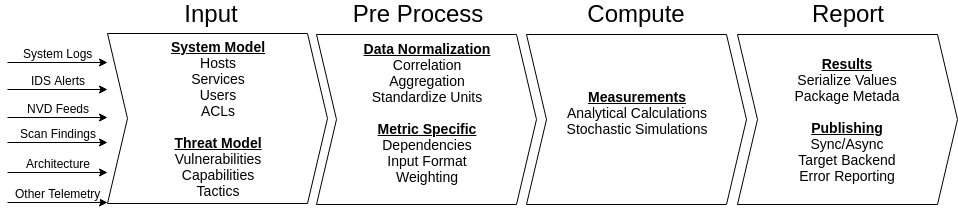
\includegraphics[width=\linewidth]{resource/img/ch_benchmarking/metric_calc_pipeline.png}
% \caption{Generalized Metric Evaluation Pipeline}
% \label{fig:automation:metric_pipeline}
% \end{figure} 
